\chapter{Bull Associations or Bull Circles}
\label{cha:Lush_Chapter_32}
\index{Bull circles|(}

The bull circle is a co-operative plan by which dairymen exchange
sires at regular intervals.\footnote{The intervals are usually two
years in length, which is about as long as they can well be without
occasionally breeding some sire to his own daughters. Sometimes the
intervals are as short as one year in order that the different owners
may get more nearly the same amount of service from each bull. The
shorter interval tends to equalize among the circle members the
differences between the bulls, but it incurs the bother of the
exchange more frequently and increases the opportunities for spreading
breeding diseases. This chapter assumes that the exchanges will take
place at intervals of two years; but, if a few words are altered, the
discussion will apply as well to cases where the exchanges are more
frequent.} In the association there are at least three, and
usually not more than five, blocks or stations. One bull is purchased for
each block or station. A block may consist of a single large herd, or it
may be a group of several small herds so located that one bull can be
used for all. After the bulls have been in service two years, they are
moved to another block. At the end of the second two years they are
moved to a third block. If there are more than three blocks in the circle,
the bulls may be moved at the end of six years to a fourth block, where
they have not been in service. If there are only three blocks in the circle
and a bull is still alive and capable of service at the end of six years, he
may be brought back to the block where he was first used. By that time
he will have been thoroughly proved. If he proved to be a very good
bull, it will be wise to use him even on those of his daughters which are
still in the first herd. If he turned out to be only an ordinary or an
inferior bull, he will be sold to the butcher. In most cases he will have
died or become sterile before he has completed six years of service. Only
rarely will the question arise as to the desirability of breeding one of
those bulls to his own daughters.

\section*{OBJECTS}
The primary object of a bull circle is to get bull service at lower
cost, or better bull service at the same cost, without running any risks
from inbreeding. If three men co-operate in a three-block circle, each
will at all times own one-third of three bulls instead of each owning
one bull. Except for death and sterility, each man will get six years of
bull service instead of two for the purchase price of one bull. A breeder
can spend less money per year in purchasing bulls even though he may
spend more money for each bull he does buy in order to get a better
pedigree or individual.

Another object is to keep dairy bulls alive until they are proved in
order that the unusually good ones among them can be used extensively
after the evidence proves them. Two years after a bull first begins his
service, his oldest daughters will be approaching 15 months of age and
will be ready to breed. At the end of four years of service his very oldest
daughters may have completed one lactation; but unless he had many
daughters from his very first services, he will be only partially proved
when it is time to move him to the third herd. Before it is time to move
him to the fourth herd he should be thoroughly proved. If he is proved
inferior, he will, of course, be sent to the butcher and his least productive
daughters will follow him. If he is proved only mediocre, he is apt
to go to the block also, since his age increases the probability that he
will soon become useless for breeding. If he proves to be very valuable,
he can be returned to the first herd for use on his own daughters and
granddaughters, thus making possible some intense linebreeding\index{Linebreeding|(} to
him.

The bull-circle plan makes it easy to pursue a consistent linebreeding
policy. For example, the first bulls in a four-block circle may all be
half brothers by some famous bull. The continued use of these bulls on
each other's daughters would tend toward producing herds which
would be almost as closely related to this outstanding sire as if they were
daughters, although it might have been quite impossible financially to
buy actual daughters of that noted bull. The amount of inbreeding in
such a plan would never get very high, tending toward but never reaching
12\nicefrac{1}{2} per cent; and all of it would be directed toward the famous
bull. If the cows in these herds are purebred, and one of the sires used
proves to be an unusually good one, it would be practical to choose the
next bulls out of the best cows in those herds where the best sire had
been used. This would lead to still further linebreeding, but with four
or five blocks in the bull circle it is unlikely that this linebreeding could
rise high enough to be dangerous, even in 30 or 40 years of steady co-operation,
provided care was always taken to select the sires from the best
cows in the herd, sired by the best of the preceding bulls. In short, the
bull circle offers almost an ideal plan for linebreeding which is fast
enough to make progress but not fast enough to be dangerous.

The bull-circle plan may also assist in a less tangible way through
the development of community spirit and co-operation. Naturally the
members of the bull circle will need to be members of a cow-testing
association if they are to take advantage of any of the objects of the
bull circle other than that of the cheaper bull service.

A ``bull club'' is merely the joining of several men together in the
co-operative purchase of a single bull. This lowers the bull cost to each
of them but does not lead to the proving of the sire since, after he has
been used two years, they will need to exchange him if he is not to be
bred to his own daughters.

\section*{INTENSITY OF INBREEDING BROUGHT ABOUT BY BULL CIRCLES}
\index{Inbreeding|(}

The upper part of Figure~\ref{fig:Lush_Figure_48} shows a pedigree with the most extreme
inbreeding which could be produced in a five-block bull circle, where
the five bulls first bought were all half brothers and each saw service in
all five blocks. A bull would rarely remain in service that long. Variations
in the sex ratio would make exceedingly rare a succession of
daughters which would result in a pedigree like this one, where X is a
descendant of all five bulls.

\begin{figure}
	\centering
    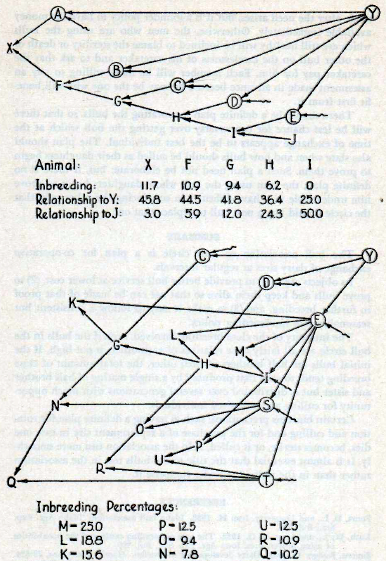
\includegraphics[width=\textwidth]{Figure_48.png}
    \caption{Some examples of extreme inbreeding which might happen in a bull
			 circle where the bulls were paternal half brothers. Upper: In a
			 five-block circle where no bull ever returned to the same block
			 and the linebreeding is purely to Y. Lower: In a three-block circle
			 where the linebreeding is first to Y and then to his son, E, who
			 is returned to be used a second time in the circle in rotation
			 with two of his sons, S and T. Encircled letters indicate sires.}
    \label{fig:Lush_Figure_48}
\end{figure}

The lower part of Figure~\ref{fig:Lush_Figure_48} shows some examples of the most
extreme inbreeding which would be apt to result in a three-block circle
where all three bulls were half brothers at the start, were used for six
years, and then it was discovered that one of them was so outstanding
that he would be used again. He would go back for service again in the
herd where he had first been used and would be mated to some of his
daughters, granddaughters and great granddaughters. There would not
be many of each. Sons of his would be placed in service in the other two
herds, where they would be used on some cows which were their paternal
half sisters and on others which were their cousins through the
paternal grandsire. The total amount of inbreeding in 10 or 12 years of
such a plan is not likely to go above 25 per cent in any individual and
probably would average only about 8 or 10 per cent. Moreover, this
inbreeding would nearly all be toward the famous sire, \textit{Y}, or his best
son, \textit{E}.
\index{Inbreeding|)}
\index{Linebreeding|)}

\section*{BUSINESS PRECAUTIONS ADVISABLE}

The title to the bull should rest in the bull association rather than
in the individual members. If each man owns one bull it is almost certain
to happen that, by the time the bulls are mature, some of them will
appear to be better individuals than others, and the owners of those
will be reluctant to exchange. If each man owns his share of all bulls,
there will not be as much of this difficulty.

A reserve fund should be provided for the replacement of bulls
which die or become sterile or which eventually prove themselves to
have been only average or less. An assessment of each block might be
made after the need arises, but it is a sounder policy to have the money
available immediately. Otherwise, the men who are using the bulls
which are still healthy will be inclined to blame the sterility or death of
the other bull on the carelessness of his caretaker and to ask that the
caretaker pay for him. Each member will be more willing to pay an
assessment made in advance because he may be the one who will benefit
first from it.

There should be a definite plan for rotating the bulls, so that there
will be less chance for controversy over getting the bull which at the
time of exchange appears to be the best individual. The plan should
also state when and how bulls should be culled as their daughters begin
to prove them. Such a plan need not be elaborate; but, if there is no
definite plan, the man using the bull whose daughters begin to prove
him undesirable may have difficulty in convincing the other men that
the circle should buy a new bull to replace that one.

\section*{SUMMARY}

The bull association or bull circle is a plan for co-operative
exchange of dairy sires at regular intervals.

Its objects are: (1) to provide better bull service at lower cost, (2) to
prove bulls and keep them alive so that use can be made of that proof
in further breeding, and (3) to make it easy to follow a consistent but
reasonably safe linebreeding policy.

The intensity of the close breeding involved, even if the bulls in the
bull circle are all fairly close relatives of each other, is not high. If the
initial bulls are half brothers of each other, the total amount of close
breeding tends toward that produced by a single mating of half brother
and sister but is distributed over several generations with much opportunity
for culling any undesired individuals.

Certain business precautions, such as having a definite plan for rotation
and culling and for the purchase of a replacement sire in case one
dies, becomes sterile, or is culled, help the association run more smoothly.
It is almost essential that the title to the bulls rest in the association
rather than in the individuals who comprise it.
\index{Bull circles|)}

\section*{REFERENCES}

\begin{hangparas}{0.5in}{1}%
Fourt, D. L., and Loughary, Ivan H. 1938. Idaho bull associations. Idaho Agr. Exp.
Sta., Bul. 223.

Lush, Jay L., and Lacy, M. D. 1932. The ages of breeding cattle and the possibilities
of using proven sires. Iowa Agr. Exp. Sta., Bul. 290.

Simons, Rodger L. 1933. Dairy development in Sweden. Hoard's Dairyman, 78:324.

Winkjer, .Joel G. 1936. Co-operative dairy bull associations. Hoard's Dairyman,
81:111 et seq.

---. 1939. Co-operative dairy bull associations. USDA, Farmers Bulletin
No. 1830.
\end{hangparas}